\chapter{MicroBlaze}

La tarjeta de desarrollo \emph{XUPV5} soporta procesadores
denomimados \emph{softcores} como el procesador
MicroBlaze\footnote{Microblaze es un \emph{soft processor} descrito en VHDL,
es una herramienta muy potente para desarrollar proyectos relacionados con
arquitecturas paralelas, codiseño, control y en toda investigación
sobre software y estudio de metodologías de desarrollo.} de
Xilinx, estos procesadores son descritos en VHDL o Verylog.

\section{Arquitectura MicroBlaze}

El procesador MicroBlaze de 32 bits ha sido desarrollado con unos requisitos muy
estrictos de ocupación y prestaciones, debido a la limitación de los recursos
disponibles en una FPGA. Soluciones arquitectónicas, como la supeescalaridad o
la supersegmentación no resultan adecuadas en un entorno lógico reprogramable,
cuando el objetivo es un diseño compacto. Del mismo modo, la frecuencia de
operación final se ve limitada por los retardos de interconexión en la FPGA.

\begin{figure}[h!]
 \centering
 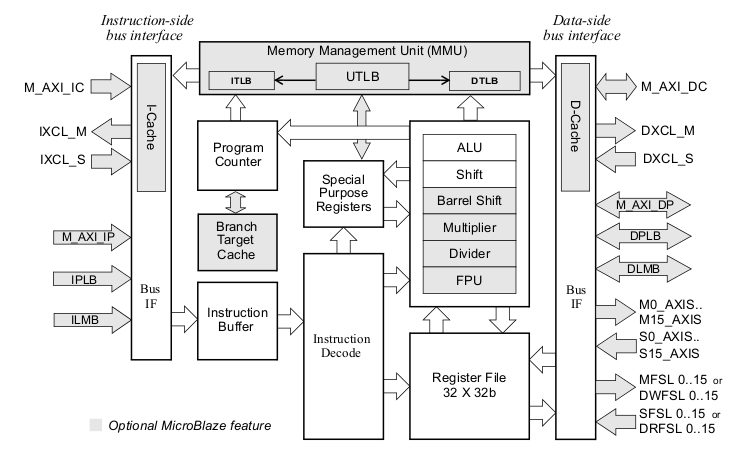
\includegraphics[scale=.55]{./figuras/ublaze.png}
 % ublaze.png: 743x451 pixel, 72dpi, 26.21x15.91 cm, bb=0 0 743 451
   \caption{Diagrama de bloques MicroBlaze}
 \label{MicroBlaze}
\end{figure}

\subsection{Conjunto de instrucciones}

La restricción de espacio fuerza a un diseño sencillo, que encaja perfectamente
con la idea de las arquitecturas tipo RISC\footnote{RISC, acrónimo de \emph{
reduced instruction set computer} es un tipo de diseño de CPU utilizado en
microprocesadores que tienen instrucciones de tamaño fijo y presentadas en un
reducido número de formatos y sólo las instrucciones de carga y almacenamiento
acceden a la memoria de datos.}, donde el limitado número de
instrucciones permite simplificar la unidad de descodificación. En el caso de
MicroBlaze, el número total de instrucciones que soporta son 87, si se
consideran diferentes las instrucciones que operan con valores inmediatos de
aquellas que realizan la misma operación con registros. Adicionalmente, cada
instrucción se ha elegido para que el tamaño de la ALU también sea reducido. Las
instrucciones que requieran un procesamiento complejo habrán de realizarse en un
hardware específico, diseñado utilizando los restantes recursos de la FPGA. El
mecanismo de conexión de estos co-procesadores con Microblaze se especifica en
el protocolo FSL(\emph{Fast Simplex Link}).

\subsection{Pipeline}


Una arquitectura RISC aumenta fácilmente su rendimiento por medio de la
segmentación \emph{pipeline}\footnote{\emph{Pipeline}, consiste en ir
transformando un flujo de datos en un proceso comprendido por varias fases
secuenciales, siendo la entrada de cada una la salida de la anterior.}. En el
caso de MicroBlaze, el número de etapas de pipeline es 3, ejecutando una
instrucción por ciclo de reloj. Como contrapartida, la segmentación debe
incorporar mecanismos para evitar los problemas relacionados con los saltos de
programa. En un salto, la pila está llena de instrucciones que no corresponden
con el flujo de ejecución.

\begin{figure}[h!]
 \centering
 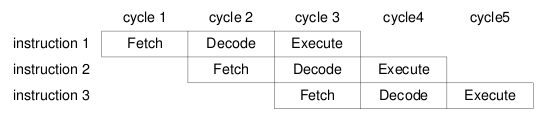
\includegraphics[scale=.60]{./figuras/ciclo.png}
 % ciclo.png: 559x121 pixel, 72dpi, 19.72x4.27 cm, bb=0 0 559 121
    \caption{3 Etapas de \emph{Pipeline: Fetch, Decode y Execute}}
 \label{Ciclo Fetch}
\end{figure}


Estos riesgos están tratados por hardware en MicroBlaze: cada vez que se produce
un salto, el pipeline se vacía cuando el salto se hace efectivo. En el
repertorio se incluyen un cierto número de instrucciones de salto que permiten
la ejecución de la instrucción que les precede, con el objetivo de reducir la
penalización de vaciado. Esta técnica es conocida como \emph{Delay Slots}.

\subsection{Registros Internos y Caché}

Las FPGAs actuales disponen de memoria distribuida con un tiempo de acceso
corto, cuando son utilizadas por la lógica cercana. Este tipo de memoria es
utilizada por MicroBlaze para materializar sus 32 registros internos, el
contador de programa y el registro de estado. Este último sólo contiene el bit
de acarreo, habilitación de cachés, indicador de estado de parada
(\emph{break}), error en el FSL y bit de excepción producida por división por
cero. Además de estos registros internos, MicroBlaze utiliza un buffer de 16
instrucciones mapeado en los registros de desplazamiento. Este recurso es
fundamental para un buen rendimiento del procesador. Por ejemplo, en caso de que
no disponer de multiplicador y/o divisor hardware, se aprovecha el tiempo que
tarda en ejecutarse esta instrucción (32 ciclos) para tener preparadas las
siguientes instrucciones.

La utilización de cachés es una práctica habitual en arquitecturas modernas; el
diseño de MicroBlaze no es una excepción. Pero en este caso, la utilización y
configuración de los tamaños de caché pueden ser fijados por el usuario. Para
ello, existe el siguiente conjunto de opciones a la hora de configurar el
procesador: habilitación de caché de instrucciones y/o datos, tamaño, rango de
direcciones y tamaño de palabra, aunque esta ultima opción solo es valida para
la caché de datos. Opciones no configurables por el usuario son tamaño
de los bloques de caché, la política de sustitución de bloques o el grado de
asociatividad de la caché.

Todas estas opciones se especifican antes de sintetizar el diseño. Las cachés
son de tipo asociativo, por lo cual es necesario el calcular el número de bits
de la dirección (\emph{tag bits}) que especifican bloques contenidos en caché,
mediante la siguente ecuación:
$$ tag bits = log_2(memoriacacheable) - log_2(tamañocaché) $$

Las cachés utilizan los bloques de RAM fijos (BRAM) que contiene la FPGA. Sin
embargo, códigos compactos también pueden mapearse en BRAM. Por lo tanto, la
utilización de cachés será necesaria en aquellos casos donde el código o los
datos utilizado por MicroBlaze residan fuera de la FPGA.

\subsection{Buses del Sistema}

MicroBlaze sigue el modelo de arquitectura Harvard, donde datos e instrucciones
son almacenados en memorias diferentes. De nuevo, gracias a la capacidad de
reconfiguracion de las FPGAs, es posible configurar el sistema con diferentes
opciones sobre los buses, pudiéndose reducir de este modo el tamaño final del
sistema. MicroBlaze utiliza el estándar \emph{CoreConnect} creado por IBM, para
conectar diferentes elementos en un circuito integrado. Un aspecto interesante
es que \emph{CoreConnect} permite reducir la carga capacitiva del bus,
repartiéndola entre varios buses. Así, se consiguen mayores rendimientos, dado
que los retardos de pistas globales son muy importantes en FPGAs.

El estándar define tres tipos de buses, cada uno con unas características de
velocidad y conectividad:

\begin{itemize}
 \item LMB (\emph{Local Memory Bus}): Bus síncrono de alta velocidad, utilizado
para conectar periféricos y los bloques de memoria interna de la FPGA. Solo
admite un maestro en su implementación para MicroBlaze y puede ser utilizado
tanto para instrucciones como para datos. Este bus es compatible con el PLB
(\emph{Processor Local Bus}) incluido en el estándar \emph{CoreConnect}, pero a
diferencia de éste, el LMB no admite varios maestros ni tamaños de palabra
diferentes a 32 bits.
 
  \item OPB (\emph{On-chip Peripheral Bus}): Bus síncrono utilizado para
conectar periféricos con tiempos de acceso variables. Soporta varios maestros y
la conectividad de muchos periféricos es sencilla gracias a su identificación
por multiplexación distribuida. Soporta transferencias de tamaño de palabra
dinámico.

 \item 	DCR (Device Control Register): Bus síncrono diseñado para una conexión
tipo anillo de periféricos con ancho de banda muy bajo. Solo soporta un maestro
y está diseñado para minimizar el uso de lógica interna.
\end{itemize}

Además de estos tres buses existe otra alternativa para comunicarse con el
procesador MicroBlaze. Se trata de un protocolo de comunicación denominado FSL
(\emph{Fast Simplex Link}) mencionado anteriormente, que permite la comunicación
con el procesador a través de sus propios registros internos. El periférico
actuaría a modo de co-procesador y la conexión se realiza de manera sencilla a
través de unos registros de desplazamiento de 32 bits de ancho. La comunicación
con estas \emph{FIFOs} se realiza con dos instrucciones específicas del
repertorio, que realizan las funciones de push y pop de estas memorias de
desplazamiento. MicroBlaze soporta hasta 16 dispositivos conectados con este
protocolo.


\subsection{Interrupciones y excepciones}

El procesador MicroBlaze contiene una línea de interrupciones, la cual al ser
activada hace que el procesador ejecute una rutina de manejo de interrupciones
que ha de ser especificada al compilador. Las excepciones se tratan de forma
similar. Cuando una de ellas ocurre, se paraliza el procesamiento de
instrucciones y se ejecuta una rutina de manejo de excepciones. En el caso de
que el sistema necesite manejar más de una interrupción, será necesario la
utilización de un periférico específico (\emph{OPB Interrupt Controller}), que
se encarga de multiplexar e identificar las diferentes fuentes de
interrupción\cite{microblaze}.

















